\documentclass[12pt]{article}
\linespread{1.3}
\usepackage{scrextend}
\usepackage{hyperref}
\usepackage{enumitem}
%\usepackage{enumerate}
\usepackage{changepage,lipsum,titlesec, longtable}
\usepackage{cite}
\usepackage{comment, xcolor}
\usepackage[pdftex]{graphicx}
  \graphicspath{{images/}, {images/stat/}}
  \DeclareGraphicsExtensions{.pdf,.jpeg,.png, .jpg}
\usepackage[cmex10]{amsmath}
\usepackage{array} 
\usepackage{subfigure} 
\usepackage{placeins} 
\usepackage{amsfonts}
\usepackage{pifont}% http://ctan.org/pkg/pifont
\usepackage{minted}

\newcommand{\cmark}{\ding{51}}%
\newcommand{\xmark}{\ding{55}}%
\newcommand{\grey}[1]{\textcolor{black!30}{#1}}
\newcommand{\red}[1]{\textcolor{red!50}{#1}}
\newcommand{\fref}[1]{Figure~\ref{#1}}
\newcommand{\tref}[1]{Table~\ref{#1}}
\newcommand{\eref}[1]{Equation~\ref{#1}}

\oddsidemargin0cm
\topmargin-2cm %I recommend adding these three lines to increase the
\textwidth16.5cm %amount of usable space on the page (and save trees)
\textheight23.5cm

\makeatletter
\renewcommand\paragraph{\@startsection{paragraph}{4}{\z@}%
            {-2.5ex\@plus -1ex \@minus -.25ex}%
            {1.25ex \@plus .25ex}%
            {\normalfont\normalsize\bfseries}}
\makeatother
\setcounter{secnumdepth}{4} % how many sectioning levels to assign numbers to
\setcounter{tocdepth}{4}    % how many sectioning levels to show in ToC

\begin{document}
\title{Regression based energy model and building energy saving literature review}
\maketitle
\tableofcontents
\newpage
% \begin{verbatim}
% Statistical Modeling of Daily Energy Consumption in Commercial Buildings
% Using Multiple Regression and Principal Component Analysis

% and its citations

% https://scholar.google.com/scholar?cites=7683762625387749884&as_sdt=5,39&sciodt=0,39&hl=en

% using all base degree day, with fuse regularization
% \end{verbatim}
\section{Motivation}
The limited availability of fossile fuels \cite{eiaNaturalGas2016,
  greentech2013}, the global warming, and other environmental
challenges brought about the global effort of energy conservation: in
the 12th 5-year plan, China set goals of reducing 16 percent energy,
and 17 percent of carbon per unit GDP; ``to move the United States
toward greater energy independence and security'', U.S. EISA act was
launched in 2007, requiring government agencies to reduce their energy
consumptions by 30\% till 2015; U.K. cut its average gas and
electricity consumption by 25\% throught increasing utility bills.

10 to 20 percent of energy cost could be saved by energy efficiency
upgrades~\cite{doeEngEff2016}. However, in order to accurately
evaluate the effectiveness of these upgrades, difference in weather,
occupancy, operation mode, etc, between pre and post retrofit needs to
be accounted for. This requires an accurate baseline energy
model~\cite{Zhang2015177}. 

In ASHRAE guideline 14, the ECM energy saving is estimated by
projecting the pre-retrofit energy consumption into the post-retrofit
period with a suitable regression model, and the saving is calculated
as the actual projected pre-retrofit consumption under post-retrofit
(weather) condition minus the post-retrofit consumption. The
predictive power of the baseline energy model determines the accuracy
of the ECM saving calculation. Such an energy baseline model could
also be used in ``determining retrofit savings, energy system fault
diagnostics, acquiring physical insight into the operating
patterns''~\cite{Zhang2015177}, and ``control strategy development, and
on-line control applications''~\cite{Zhang2015177}

In addition to the predictive power, some baseline model also provides
separate the whole building energy into different end uses such as
heating, cooling, and baseload~\cite{fels1986prism, leanEng,
  firstViewUnder2016, wytock2013contextually}. This could be used in
energy use benchmarking~\cite{leanEng}, identifying energy retrofit
opportunities~\cite{leanEng, wytock2013contextually}, and encourage
energy saving behaviors~\cite{wytock2013contextually}.

In this study, I will review a series of black-box or gray-box
data-driven energy baseline methods, and compare their predictive
performance of the aggregated consumption, and or the end-use
consumption.

% An energy signature model (ES) of a building contains parameters that
% represents its energy performance~\cite{hammarsten1987critical}. The
% model parameters are usually estimated with statistical analysis
% instead of simulation. The ES could be used to predict building energy
% consumption or estimate building
% parameters~\cite{hammarsten1987critical}.

% \subsection{Goal}
% The goal of the do
% Deliver a method to perform weather normalization on a portfolio, with
% the following good features:
% \begin{itemize}
% \item transformed / cleaned input
% \item Ensemble method that combines multiple algorithms to obtain
%   better predictive performance than could be obtained from any of the
%   constituent learning algorithms alone
% \end{itemize}

% The method will be tested on a large data set to ensure its
% robustness.

% Based on the identified limitations of the ASHRAE method, the thesis
% aims to then propose a more accurate / robust method for weather
% normalization and energy saving calculation, and the proposed method
% will be tested on a large scale building stock (the GSA portfolio with
% 1700 buildings).

\section{Background}
In ASHRAE Handbook-Fundamentals, approaches to estimate building
energy usage are broadly classified into forward and inverse method. A
system contains three components: the input, the system structure, and
the output~\cite{edition2013ashrae}. The forward approach is given the
input and the system structure to predict the output. It is based on
the ``engineering principles'' and the model is a ``physical
description'' of the building and its sub
systems~\cite{edition2013ashrae}. It is advantageous for evaluating
the energy performance of the design and analysis stage but requires a
lot of physical inputs. The inverse model approach aims to estimate
the system parameters given the input and output. It is only
applicable to existing systems with actual measured data. The inverse
models are ``more accurate predictors of future system performance
than forward method''~\cite{edition2013ashrae} because it captures
more accurately the ``as-built'' system information, the data are more
ready to get, and it is easier to be automated and thus is good for
the analysis of large building portfolio~\cite{rabl1992energy}. The
data-driven method is flexible as it could model both whole building,
and equipment such as pumps, fans, chillers, and
boilers~\cite{edition2013ashrae}. As a result, the inverse models are
receiving increasing attentions.

In literature, the topic is referred to as: whole building or building
baseline models~\cite{granderson2014evaluation, reddy1997baselining,
  kissock2008methodology, dong2005applying, Zhang2015177},
weather-adjusted index of consumption~\cite{fels1986prism}, energy
signature model~\cite{rabl1992energy, hammarsten1987critical}, inverse
(energy) model~\cite{kissock2003, abushakra1997inverse, Zhang2015177},
data-driven (energy) models~\cite{Zhang2015177}, energy prediction
model~\cite{mocanu2016deep, Yu20101637, dong2005applying}.

The models could be used for building load / demand / consumption
forcasting~\cite{dong2005applying, solomon2011forecasting, Yu20101637,
  mocanu2016deep, hammarsten1987critical}, calculation of measured
energy savings from energy conservation retrofits~\cite{haberl1994bin,
  edition2013ashrae, kissock2008methodology, kissock2003,
  fels1986prism}, evaluating building energy
performance~\cite{abushakra1997inverse}, building parameter
estimation~\cite{hammarsten1987critical}, energy end use
disaggregation~\cite{leanEng, fels1986prism, wytock2013contextually},
assist the ``identification of energy saving opportunities and
recommend the types of energy efficiency measures''~\cite{leanEng}.

% Common environmental variables used in the models are dry-bulb
% temperature, humidity, and solar
% radiation~\cite{dong2005applying}. Former studies has identified that
% the outdoor dry-bulb temperature is the most important predictor at
% monthly and daily time scale~\cite{reddy1997baselining} (although,
% this assertion needs to be further validated).

% This study thus focuses on the
% single variable regression method (the black-box approach) with
% weather as the independent variable.
%
% fixme: where did it say so
%
\section{Related works: Models}
\begin{table}[h!]
  \centering
    \tiny
  \begin{tabular}{p{3.0cm}|p{0.7cm}|p{0.7cm}|p{0.7cm}|p{0.7cm}|p{0.7cm}|p{0.7cm}|p{0.7cm}|p{0.7cm}|p{0.7cm}|p{0.7cm}|p{0.7cm}|p{0.7cm}|p{0.7cm}}
    \hline
    paper&linear &piecewise &SVM&kernel&Gaussian process&Gaussian mixture&ANN&PAM&mean-week&day-time-temperature&LBNL&Decision Tree&PCA\\
    \hline
    \hline
    Baselining methodology for facility-level monthly energy
    % usepart 1: Theoretical aspects~\cite{reddy1997baselining}&VBDD,2p MMT& 3p  5p change point model &  & &&&&\\
    usepart 1: Theoretical aspects~\cite{reddy1997baselining}&\cmark&\cmark&  & &&&&&&&&&\\
    \hline
    PRISM: an introduction~\cite{fels1986prism}&\cmark&&&&&&&&&&&&\\
    \hline
    ENERGY STAR Score~\cite{energyStarDoc}&\cmark&&&&&&&&&&&&\\
    Comparisons of inverse modeling approaches for predicting
    building energy performance~\cite{Zhang2015177}&  &\cmark&  & &\cmark&\cmark&\cmark&&&&&&\\
    \hline
    Applying support vector machines to predict building
    energy consumption in tropical region~\cite{dong2005applying}&&&\cmark&&&&&&&&&&\\
    \hline
    Kernel regression for real-time building energy
    analysis~\cite{brown2012kernel}&&&&\cmark&&&&&&&&&\\
    \hline
    Deep learning for estimating building energy
    consumption~\cite{mocanu2016deep}&&&&&&&\cmark&&&&&&\\
    \hline
    Evaluation of the Predictive Accuracy of Five Whole
    Building Baseline Models&&\cmark&&&&&&\cmark&\cmark&\cmark&\cmark&&\\
    \hline
    Forecasting Energy Demand in Large Commercial Buildings
    Using Support Vector Machine Regression&&&\cmark&&&&&&&&&&\\
    \hline
    % Saving Electrical Energy in Commercial Buildings
    % ~\cite{case2012saving}&&&&&&&&&&&&&\\
    A decision tree method for building energy demand modeling~\cite{Yu20101637}&&&&&&&&&&&&\cmark&\\
    \hline
    Statistical Modeling of Daily Energy Consumption in
    Commercial Buildings Using Multiple Regression and Principal
    Component Analysis~\cite{claridge1992statistical}&&&&&&&&&&&&&\cmark\\
    \hline
    Principal component analysis in building energy efficiency
    rating system for apartment housings~\cite{jung2014principal}&&&&&&&&&&&&&\cmark\\
    \hline
  \end{tabular}
  \caption{matrix of related works energy prediction baseline model}
  \label{tab:work}
\end{table}
\FloatBarrier
\begin{table}
    \tiny
  \begin{tabular}{p{6cm}|p{1cm}|p{1cm}|p{1cm}}
    \hline
    paper&linear &piecewise &contextual learning\\
    \hline
    \hline
    Contextually Supervised Source Separation with Application
    to Energy Disaggregation~\cite{wytock2013contextually}&&&\cmark\\
    \hline
    PRISM: an introduction~\cite{fels1986prism}&\cmark&&\\
    \hline
    LEAN Energy Analysis Using Regression Analysis to Assess
    Building Energy Performance~\cite{leanEng}&&\cmark&\\
    \hline
  \end{tabular}
  \caption{matrix of energy disaggregation baseline model}
  \label{tab:workDisagg}
\end{table}
\FloatBarrier
% \begin{table}[h!]
%   \centering
%     \footnotesize
%   \begin{tabular}{p{1cm}|p{3cm}|p{3cm}|p{5cm}|p{1cm}}
%     \hline
%     method&weather input&consumption input&form&source\\
%     \hline
%     \hline
%     CBDD  &heating / cooling degree day&monthly mean daily utility bill reading&$Y = \alpha + \beta \cdot DD(\tau)$&\cite{reddy1997baselining}\\
%     VBDD  &heating / cooling degree day&monthly mean daily utility bill reading&$Y = \alpha + \beta \cdot DD(\tau)$&\cite{reddy1997baselining}\\
%     &&&$Y = \alpha + \beta_h \cdot DD(\tau_h) + \beta_c \cdot DD(\tau_h)$&\\
%     \hline
%     MMT-1p&monthly mean temperature    &..&$\bar{Y}$&\cite{reddy1997baselining}\\
%     \hline
%     MMT-2p&monthly mean temperature    &..&$Y = \alpha + \beta \cdot T$&\cite{reddy1997baselining}\\
%     \hline
%     MMT-3p&monthly mean temperature    &..&$Y = Y_{cp} + RS \cdot (T - X_{CP})^+$&\cite{reddy1997baselining}\\
%           &                            &  &$Y = Y_{cp} + LS \cdot (T - X_{CP})^-$&\cite{reddy1997baselining}\\
%     \hline
%     MMT-4p&monthly mean temperature    &..&$Y = Y_{cp} + RS \cdot (T - X_{CP})^+ + LS \cdot (T - X_{CP})^2$&\cite{reddy1997baselining}\\
%     \hline
%     MMT-5p&monthly mean temperature    &..&$Y = Y_{cp} + RS \cdot (T - X_{CP, h})^+ + LS \cdot (T - X_{CP, c})^2$&\cite{reddy1997baselining}\\
%     \hline
%     \hline
%   \end{tabular}
%   \caption{Weather normalization method matrix}
%   \label{tab:method}
% \end{table}
% \FloatBarrier

There are different aspect to categorize the models found in
literature.
%A series of methods were developed in the 80s and 90s of last century.
 
Based on the representation of outdoor temperature, the models are
categorized as: mean temperature model, degree-day based model, and
transformed hourly temperature (either with radio basis function, or
with exponential weighting). 

The mean temperature model could be sub-divided into 1p to 5p models
based on the number of parameters involved. The degree-day models can
be subdivided into constant-base degree day (CBDD) model and
variable-base degree-day model (VBDD). The heating or cooling degree-day is
calculated with respect to a certain temperature. This temperature is
called ``balance point temperature''~\cite{edition2013ashrae}, ``base
of the degree-day''~\cite{edition2013ashrae}, ``break-even
temperature''~\cite{fels1986prism}, or ``reference
temperature''~\cite{fels1986prism, Zhang2015177, fels1986prism}. It is
defined as the outdoor temperature at which the heat loss equals to
the internal and external heat gain, and no heating or cooling energy
is needed~\cite{edition2013ashrae}.
%
CBDD uses a fixed balance point temperature for the heating or cooling
degree-day calculation, which is usually 65F. As the balance point
temperature is usually not the same for all
buildings~\cite{fels1986prism} and the selection of a proper balance
point temperature could greatly affect the result of saving
calculation, Fels et al.\ developed the VBDD model that chooses the
balance point temperature with the highest $R^2$~\cite{kissock2003}.
%fixme citation fels1986prism needs to be verified

Most of the methods are regression based. Based on the type of
regression, the methods can be categorized into linear regression,
segmented (piecewise) linear regression, Gaussian process regression
model, Gaussian Mixture regression model~\cite{Zhang2015177}, Kernel
regression~\cite{brown2012kernel}, SVM
regression~\cite{dong2005applying}, ANN etc.. Linear regression models
in the current context refer to the model with the form of
(\eref{eq:linearReg}) where $y$ is the dependent variable,
$\mathbf{x}$ is the independent (explanatory) variable vector,
$\mathbf{w}$ is the model parameter vector, $b$ is the intercept term,
and $\epsilon$ is the error or noise. The VBDD or CBDD method falls
into this category.
\begin{equation}
  \label{eq:linearReg}
  y = \mathbf{w}^T\mathbf{x} + b + \epsilon
\end{equation}
The the ordinary least square method is commonly used to estimate the
regression model parameters where the sum of the squared error is
minimized~\cite{ordinaryLeastSquareWiki2016}. The method assumes the
data has iid Gaussian noise
($\epsilon \sim \mathcal{N}(0, \sigma^2)$), as it corresponds to the
maximum likelihood estimate of the model parameters. However, the iid
Gaussian assumption is violated as 1) the observed energy consumption
cannot be negative, thus the error of the negative part is
truncated~\cite{rabl1992energy}. The Tobit model is more suitable in
this case~\cite{TobitWiki2016}. Rabl and Rialhe observed a 10\%
difference in the slope term estimate between the least square method
and the Tobit model method. Another approach to account for the
non-Gaussian error is presented in ~\cite{huang2003short}.

Segmented or piecewise regression could refer to partitioning the
independent variable into intervals and solve each segment with linear
regression, or partitioning the independent
variables~\cite{segmentRegWiki2016}. The segmented regression in the
current context refers to the former. The change-point models is in
this category, but it has an additional constraint: adjacent segments
are continuous.

Kernel regression or kernel smoothing method makes prediction with a
``weighted average of nearby data items, with the weights being
controlled by a kernel function''~\cite{brown2012kernel}. Brown et
al.\ presented a novel approach using kernel regression to predict
hourly energy consumption.

SVM could be used in both classification and regression settings. The
advantage of SVM includes 1) the Lagrangian dual is kernelizable, and
thus has better guarantee to achieve a ``smoother'' solution that
generalizes better to unseen data 2) through proper regularization, it
could provide a sparse solution. Some examples include
~\cite{dong2005applying, solomon2011forecasting}.

A series of ANN based models are developed to predict hourly
consumption during the ASHRAE ``great energy predictor shootout''
phase I~\cite{kreider1994predicting} and II~\cite{haberl1998great}
competitions. Its goal is to find ``the most effective empirical or
inverse regression models for modelling hourly whole-building energy
baselines for purposes of measuring savings from energy conservation
retrofits''~\cite{haberl1998great}. In phase I, 4-6 months of
electricity hourly data and environmental data (``temperature,
humidity, solar flux and wind''~\cite{mackay1996bayesian}) are given
as inputs~\cite{brown2012kernel}. In phase II, ``two sets of measured
hourly pre-retrofit and post-retrofit data from buildings
participating in a revolving loan program in Texas'' are given as
input~\cite{haberl1998great}. % ``A supervised
% neural network is a non-linear parameterized mapping from an input $x$
% to an output $y = y(x; w)$''~\cite{mackay1996bayesian}
% . It could be used for regression or classification. A two layer
% neuron network could have the following form
% \begin{equation}
%   \label{eq:ann2}
%   h_j  = f^{(1)}(\sum_{k}^{(1)}w_{jk}x_k + \theta_j^{(1)}); y_i = f^{(2)}(\sum_jw_{ij}^{(2)}(\sum_jw_{ij}^{(2)}h_j + \theta_i^{(2)}
% \end{equation}
Comparing with linear regression, the hidden layer provides it with
more flexibility~\cite{mackay1996bayesian}. The winner for phase I is
an ANN with the Automatic Relevance Determination prior
(ARD)~\cite{mackay1996bayesian}. The winner for phase II is ANN with
Wald’s test~\cite{dodier2004statistical}.

The output of the models can be ``actual savings'' or ``normalized
savings''. The method developed by Kissock and adopted by ASHRAE
guideline measures the ``actual saving'', which project the
consumption of the baseline model to the post-retrofit period. The
PRISM method and the one Energy Star uses ~\cite{pmWeather} measures
the normalized savings (NAC): the ``annual energy consumption during a year
of average weather condition''~\cite{reddy1997baselining}.

Based on whether the model contains the ``time lag'' term, they are
classified as steady-state models, and dynamic
models~\cite{edition2013ashrae}. Steady-state models assumes ``(i) the
building is a linear system and (ii) the driving terms are periodic
(and the interval for the data analysis.  is a multiple of this
period)''~\cite{rabl1992energy}. It is sufficient for the analysis on
the daily or monthly level as most buildings have a operation cycle of
24 h~\cite{rabl1992energy}. For hourly or sub-hourly data, the
assumption of the least square method will be violated, as the noise
of consecutive measurements are not
independent~\cite{hammarsten1987critical}.

\section{Model evaluation}
This section discusses the issues and concerns about model evaluation
in the following aspects.
\subsection{Robustness to noise in the input data}
We are concerned with the influence of the noise in the input data on
the model estimate, thus one important factor is the robustness with
respect to noisy input data. For example, hammarsten showed that
random errors in degree-day input could result in a systematic lower
estimate of the slope term~\cite{hammarsten1987critical}. Some model
regularization techniques could reduce the impact of noisy input and
make accurate predictions: Mackay used a ARD prior to reduce the
impact of junk inputs~\cite{mackay1996bayesian}, Dodier
and Henze used Wald's test~\cite{dodier2004statistical}.

\subsection{Predictive power and physically meaningful}
Two main usage of the baseline models are 1) predicting energy
consumption and 2) providing physical insights and suggest possible
energy retrofit opportunities. Thus the predictive power and
physically meaningful are two criteria for evaluating which is a
suitable model.

The parameters of most black-box models tends to lack physical
meanings, those of the calibrated simulation are based on the building
physical conditions. The grey-box model with simplified building
specification~\cite{brown2012kernel}.

A model with high predictive power could produce more accurate
estimate of the energy consumption. This is crucial in the ECM energy
saving estimation. For model selection, the ASHRAE guideline 14
recommend the model with the best $R^2$ or $CV(RMSE)$. The following
metrics are used to evaluate the predictive power of the model
\begin{table}[h!]
\centering
\tiny
\begin{tabular}{c|p{5cm}|c}
  \hline
  Metric  &definition                       &source              \\
  \hline
  \hline
  $R^2$   &                                 &\cite{edition2013ashrae}\\
  \hline
  RMSE    &Root Mean Squared Error          &\cite{edition2013ashrae}\\
  \hline
  CV-RMSE &Coefficient of variance of RMSE  &\cite{edition2013ashrae, brown2012kernel}\\
  \hline
  NMBE    &Net Mean Bias Error              &\cite{edition2013ashrae}\\
  \hline
  Net Determination Bias& bias of the computation&~\cite{edition2013ashrae}\\
  \hline
  SE      &Standard Error                   &\cite{reddy1997baselining, hammarsten1987critical}\\
  \hline
  PI      &Confidence Interval (90\%)       &\cite{reddy1997baselining}\\
  \hline
  MAE     &Mean Absolute Error              &\cite{wytock2013contextually}\\
  \hline
  Cross Validation&``a model validation technique for assessing how the results of a statistical analysis will generalize to an independent data set''~\cite{cvWiki2016}&\cite{brown2012kernel}\\
  \hline
  median absolute percentage error&&\cite{granderson2014evaluation}\\
  \hline
\end{tabular}
\caption{Model evaluation metric for predictive power}
\label{tab:eval}
\end{table}
\FloatBarrier

  \begin{itemize}
  \item cross validation: K-fold cross validation~\cite{case2012saving}
  \item SE: standard error of the coefficient. It ``describes how much
    of the variance in the dependent variable is described by the
    model''~\cite{hammarsten1987critical}. It reflects ``how
    accurately the regression model is able to identify the individual
    model coefficients''~\cite{reddy1997baselining}. It is similar to
    the p value for the coefficients.
  \item standard deviation of the noise~\cite{hammarsten1987critical}
    An example of daily vs weekly data comparison is shown in
    ~\cite{hammarsten1987critical}, demonstrating the $R^2$ by
    itself is not sufficient to evaluate the model with different
    time step and the difference in standard deviation of the
    noise needs to be adjusted: in the example, the weekly model
    have higher $R^2$ than the daily model, but that's a result of
    decreased variance of the
    data~\cite{hammarsten1987critical}. If the daily model
    predicted aggregated monthly consumption is actually more
    accurate than the monthly model
    prediction~\cite{hammarsten1987critical}.
  \item Coefficient of determination or $R^2$: it evaluates how well a
    model fits the data~\cite{reddy1997baselining}.
    \begin{equation}
      \label{eq:r2}
    1 - \frac{\sum_i(y_i - \bar{y})^2}{\sum_i(y_i - \hat{y_i})^2}
    \end{equation}
\item CV-RMSE: evaluates the mean variation in the data that is not explained by the model~\cite{reddy1997baselining}.
  $$CV-RMSE = \frac{RMSE}{\bar{y}} \cdot 100$$
\item NDB: The term ``bias'' used here is different from that in
  statistics (which is guaranteed to be zero by doing regression). net
  determination bias. In ASHRAE standard, the ``Net determination bias
  should be no more than 0.5\% for regression models for
  whole-building and retrofit isolation approaches'', later in the
  standard, it says the net determination bias should be less than
  ``0.005\%''. Also, it seems that NDB could be negative.
  $$NDB = \frac{\sum(y_i - \hat{y_i})}{\sum y_i}$$~\cite{Kim2015}.
\item PI: confidence interval, by convention use the 90\%
  level~\cite{reddy1997baselining}. However, in 3P change point model,
  the residual on different side of the change points are found to be
  un-equal for a lot of cases (non-uniform model residual
  problem)~\cite{reddy1997baselining}, so the PI is not suitable for
  3P change point.
\end{itemize}

To apply the model to energy audit, the physical meaningfulness is an
important part. ANN has good prediction power, but its parameters are
meaningless regarding the building's physical condition. There are
also cases when the model only corresponds to the physically condition at times.
% \begin{itemize}
% \item The bias of the estimated parameter~\cite{hammarsten1987critical} ??
For example, in the case of simultaneous heating and cooling, the base
load could be over-estimated~\cite{rabl1992energy}. In the following
example, the solid line is the total consumption (steam), and the true
heating and cooling balance point temperature (estimated with
sub-meter data) are the dashed line. This example demonstrated that
the model estimated ``breakpoint temperature'' might not correspond to
the true balance point temperature with actual physical meaning.
\begin{figure}[h!]
  \centering
  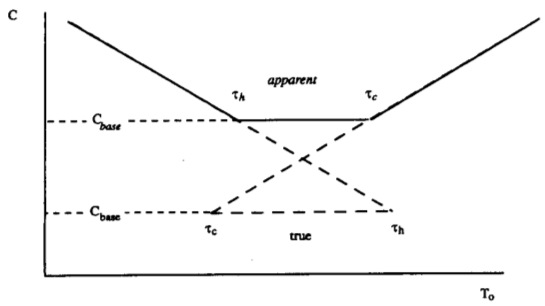
\includegraphics[width=0.5\textwidth]{images/apparentVsTrue.png}
  \caption{The true balance point vs the apparent~\cite{rabl1992energy}}
  \label{fig:asf}
\end{figure}
\FloatBarrier
\subsection{Performance under small training data set}
There are a lot of cases in which we do not have enough training data
points for the baseline period: two consecutive retrofit are close in
time and we want to evaluate the incremental saving from one retrofit
to another; predicting energy consumption for a new building. Thus the
performance under small amount of data could be another metric to
evaluate models.

% \begin{itemize}
% \item the MMT-5p is reduced to MMT-4p if the heating and cooling ``cross-over'', but in this case, the ``base load'' cannot be calculated~\cite{reddy1997baselining}
% \item VBDD: ``most suitable for shell-dominated buildings such as
%   residences and small commercial buildings wherein energy use is not
%   strongly influ- enced by the nonlinear behavior exhibited by
%   chillers, refriger- ation equipment, and boilers''~\cite{reddy1997baselining}
% \end{itemize}

% \subsection{Background: how bad the current approaches are}
% The thesis aims to show the following limitations on the ASHRAE
% recommended standard for weather normalization in energy retrofit
% savings calculations
% \begin{itemize}
% \item Lack of testing / validation of the model on large number of buildings. 
% \item The metric for evaluation the goodness of the ``fit'' needs to
%   account for different fuel types: From a preliminary study using the
%   portfolio monthly energy consumption data in the GSA project, the
%   author found that the ``errors'' (CV(RMSE)) in the gas consumption
%   calculation is much more than those in the electric calculation.
% \item Lack input regularization / transformation: billing period error
%   influences the energy consumption data; pre-processing data to
%   account for difference in error rate along the temperature. % \end{itemize} 
\section{Related work: Packages / software tool}
This section reviews the method, input, output, time-interval and
other features of available software or packages that produces
baseline models.
\begin{table}[h!]
  \centering
  \tiny
  \begin{tabular}{c|p{1,5cm}|p{2cm}|p{4cm}|p{4cm}|p{1cm}|p{0.5cm}}
    \hline
    tool&author&methods&input&output&time step&source\\
    \hline
    \hline
    E-Tracker&Kelly Kissock et al.\ &4p or 5p change point model&meter reading date, electricity and thermal energy consumption, peak electrical demand, average daily outdoor temperatures&saving, baseline model parameters, $R^2$, CV-RMSE&monthly&~\cite{etracker2003}\\
    \hline
    PRISM&Fels et al.\ &VBDD&one year utility bill, average daily temperature&$R^2$, CV-RMSE of NAC&monthly&~\cite{fels1986prism}\\
    \hline
    ECAM&William Koran&linear (2p) and 3-6p change-point &energy data, temperature of closest weather station, or TMY3&Projected Baseline Energy (pre), Measured Energy (post), Energy Saving (avoided consumption), CV-RMSE, NDB, 95\% confidence interval of the output, pre and post period NAC&daily or hourly&~\cite{ecamPnnl2016}\\
    \hline
    First View&NBI&unknown&utility bill, building characteristics&LEAN plot, ``spectrum plot''&monthly&~\cite{firstViewUnder2016}\\
                \hline
  \end{tabular}
  \caption{tools}
  \label{tab:tool}
\end{table}
\FloatBarrier
\begin{itemize}
\item{E-Tracker}
The portfolio manager energy star uses a method based on the
E-tracker~\cite{pmWeather}.

The flowing are the screen shots of the software with its sample input
data. From the tool, it seems the 4p model implemented by this model
does not rule out the case of the model with left side slope up and
right side slope down.
\begin{figure}[h!]
  \centering
  \begin{subfigure}
  \centering
  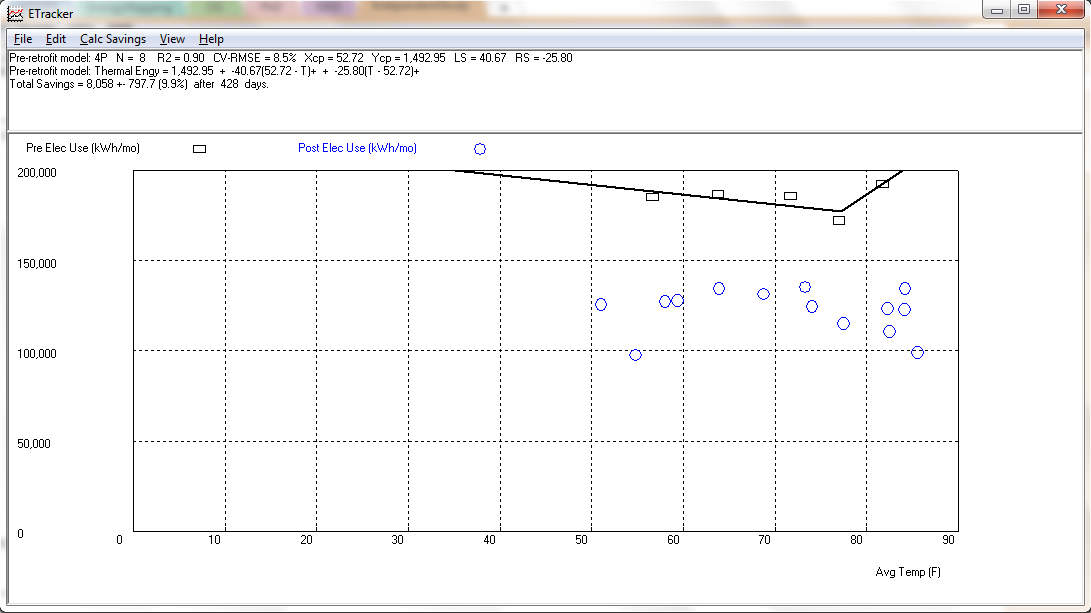
\includegraphics[width=0.6\linewidth]{images/etracker_model_elec.png}
  \caption{E-tracker electric baseline model}
  \label{fig:elec_etracker}
\end{subfigure}
~
\begin{subfigure}
  \centering
  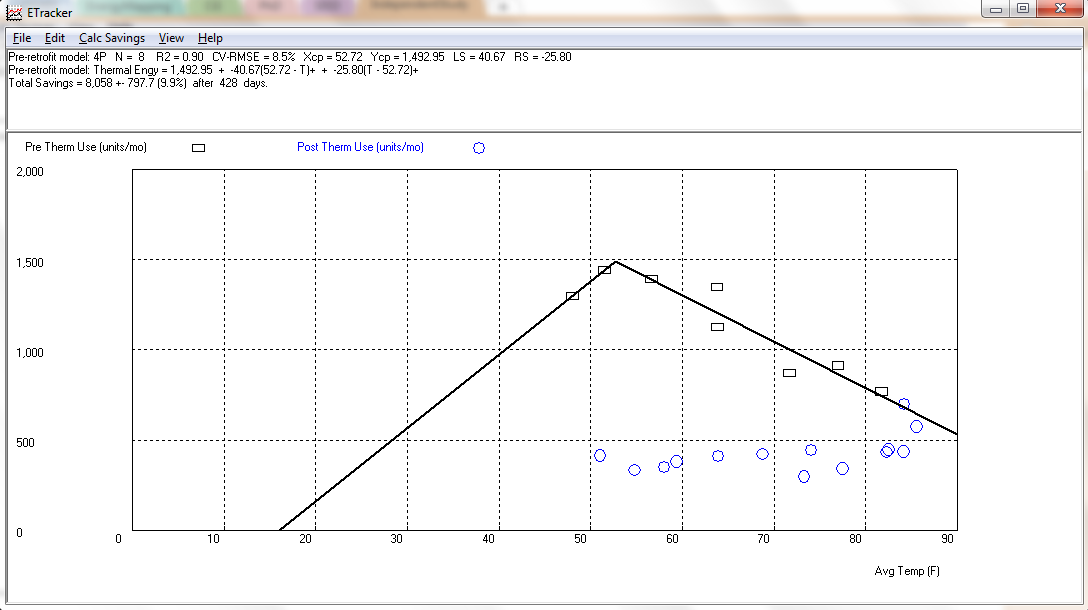
\includegraphics[width=0.6\linewidth]{images/etracker_model_gas.png}
  \caption{E-tracker gas baseline model}
  \label{fig:heatpower}
\end{subfigure}
\end{figure}
\FloatBarrier
\item First View: from the description in ~\cite{firstView2016}, the
  input is described as ``monthly utility bills and a few building
  characteristics'', and from ~\cite{firstViewUnder2016}, the method
  to calculate the baseload, heating, cooling load are not clear, or
  does not seem to be likely what the tool is actually doing. They
  claimed the electric base load is ``calculated as the sum of
  lighting, plug loads, year-round fans and pumps, consistent process
  loads and electric water heating'', but this seems to be impossible,
  unless they ask users to directly input the consumption of those
  components. The heating and cooling load is calculated from
  ``analyzing the estimated internal gains, overall heat transfer
  coefficient, and modeled equipment efficiencies of a building''. Gas
  base load is calculated by from ``summer gas use''. The method of
  separating different end use described in the First View document
  does not appear in other literature I've read so far. 

  In addition to creating a LEAN energy plot of heating, cooling, base
  gas and base electric plot, they also provides a ``spectrum'' of
  energy signature plot (energy consumption vs temperature). There's
  no documentation about how it is computed.
  \begin{figure}[h!]
    \centering
    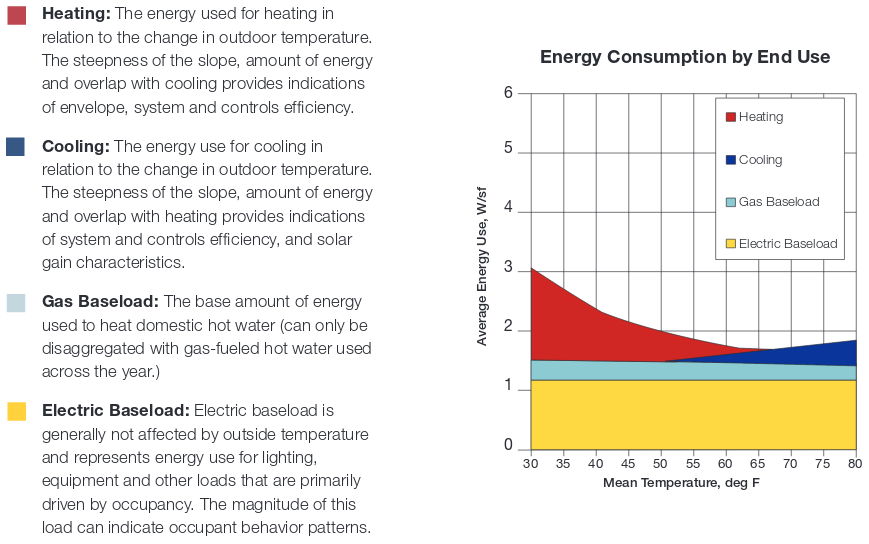
\includegraphics[width=0.7\textwidth]{images/nbiLean.png}
    \caption{First View LEAN plot~\cite{firstViewUnder2016}}
    \label{fig:nbiLean}
  \end{figure}
  \FloatBarrier
  \begin{figure}[h!]
    \centering
    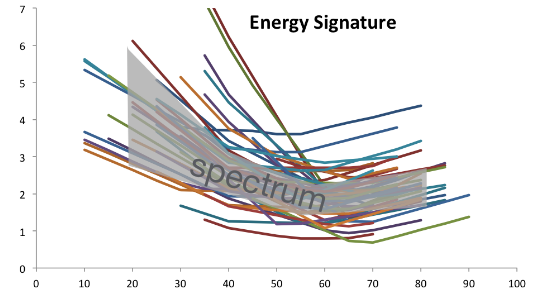
\includegraphics[width=0.7\textwidth]{images/nbiSpec.png}
    \caption{First View Spectrum Plot}
    \label{fig:nbiSpec}
  \end{figure}
  \FloatBarrier
\end{itemize}
\section{Summary of individual papers}
\subsection{A Critical Appraisal of Energy-Signature Models~\cite{hammarsten1987critical}}
Energy Signature (ES) are parameters in a energy-balance model. ES can
describe the energy performance. Other equivalent terms include
Equivalent Thermal Parameter (ETP), and Building Element Vector
Analysis (BEVA).

The paper reviewed some energy
signature (ES) models. Static ES models could be used in cases with
time-step at least one day. The author define the ES model to be a set
of parameters that describe the energy performance of a building in an
energy-balance model.

Models reviewed are:
\begin{itemize}
\item static two-parameter: assuming constant / stable indoor temperature
  \begin{equation}
    \label{eq:2p-model}
    Q = Q_0 - LT_o
  \end{equation}
\item static two-parameter with indoor and outdoor temperature
  \begin{equation}
    \label{eq:2p-model-intercept}
    Q = Q_0 - L(T_i - T_o)
  \end{equation}
\item dynamic model with lag term (the same variable in previous N
  time steps), $I$ is solar radiation, $Q_0$ is the constant power
  loss or gain, $Q$ is power.
  \begin{equation}
    \label{eq:dyn-model}
    \sum_{k = 0}^N a_k T_i(t - k) + \sum_{k = 0}^N b_k T_o(t - k) + \sum_{k = 0}^N c_k I(t - k) - \sum_{k = 0}^N d_k Q(t - k) = Q_0
  \end{equation}
\end{itemize}

input variables:
\begin{itemize}
  % lookup
\item environment: outside air temperature ($T_o$), indoor temperature, solar radiation
  ($T_i$), solar aperture ($S$).
\item energy: power
\end{itemize}

\subsection{A BIN METHOD FOR CALCULATING ENERGY CONSERVATION RETROFIT SAVINGS IN
COMMERCIAL BUILDINGS~\cite{haberl1994bin}}
The author pointed out that even if change-point models accounted for
some non-linear relationship between temperature and energy
consumption, there are buildings that change-point models do not fit
well. The paper aims to improve the existing model and presented a
method of using ``hourly bin'' to calculate retrofit energy savings,
the result is tested in two buildings.

% The author categorizes existing approaches into regression models,
% calibrated simulation, and simplified system model. 

Required data include: at least nine months pre-retrofit hourly energy
data, and hourly temperature data. Energy data include electricity, AHU
electricity, chilled water, hot water energy consumption.

A box-whisker-mean plot is used: it is similar to the box plot, except
that the high and low end of the whiskers are the 90th and the 10th
percentile (or the authors might have remembered it wrong).  The
method splits the energy into two types: weather independent and
weather dependent, for the former, the x axis is time of the day; for
the latter, the x axis is the outdoor air temperature.

\begin{figure}[h!]
  \centering
  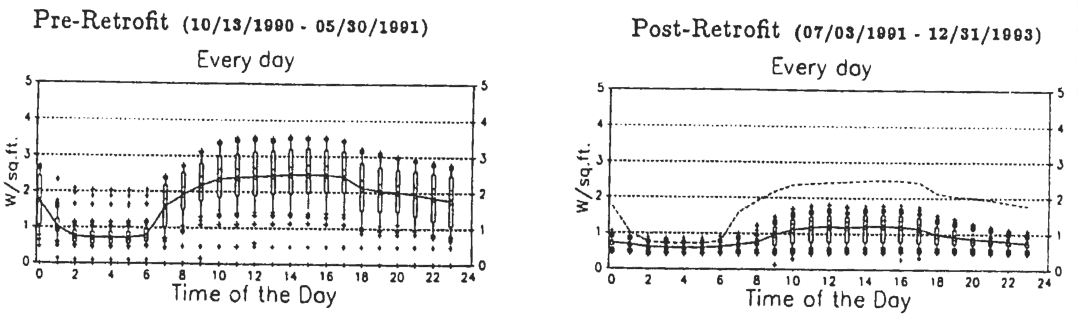
\includegraphics[width=0.7\textwidth]{images/weather_independent.png}
  \caption{weather independent energy model}
  \label{fig:weather_independent}
\end{figure}
\begin{figure}[h!]
  \centering
  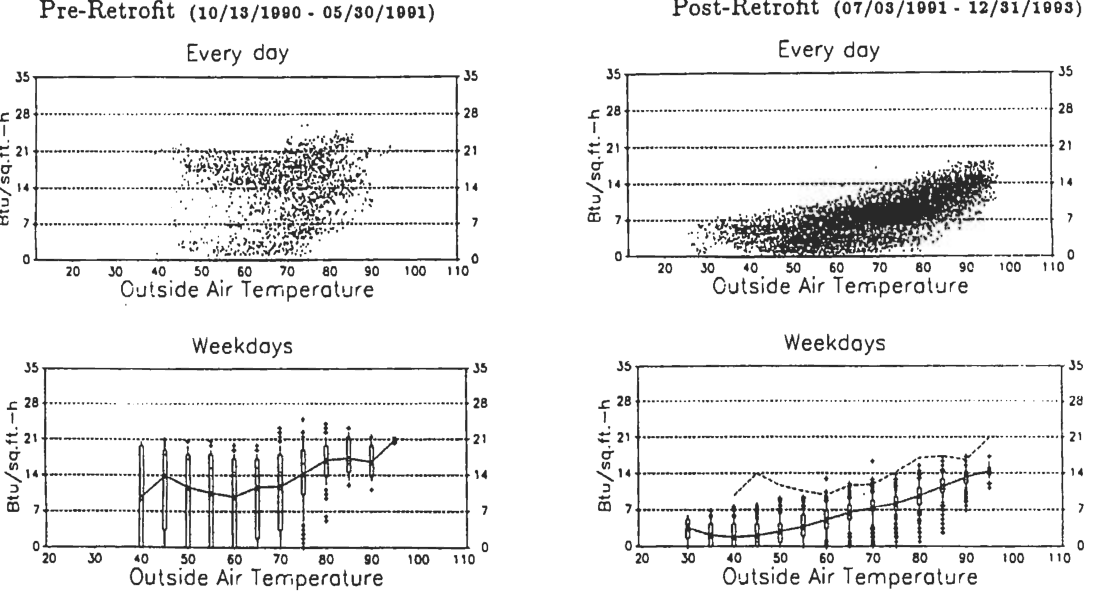
\includegraphics[width=0.7\textwidth]{images/weather_dependent.png}
  \caption{weather dependent energy model}
  \label{fig:weather_dependent}
\end{figure}
\FloatBarrier

The saving is determined with \eref{eq:save_bin_non}.
$E_{pre_{i, j}}$ is the pre-retrofit model predicted post-retrofit use
for model $i$ hour $j$ in the non-weather dependent case, temperature
bin $j$ for the weather dependent case.
\begin{equation}
  \label{eq:save_bin_non}
  \sum_{i = 1}^n\sum_{j = 1}^m (E_{pre_{i, j}} - E_{post_{i, j}})
\end{equation}

In the non-weather dependent (schedule dependent) case.  The saving is
determined by comparing the hourly average consumption for each model
in pre-retrofit period, and post-retrofit period. Outliers are removed
as follows: when a day has entire 24h consumption below the 10th
percentile or above the 90th percentile.

A separate model (indexed by $i$) is fit to a different operation mode
for both cases. Bins are selected so that the interquartile range is
below a threshold (?? is this reasonable). The models are evaluated
with $R^2$, Coefficient of Variance, and Mean Bias Error. Althrough,
it seems the authors are mainly selling the fact that the bin method
have lower Coefficient of Variance, without mentioning that they have
higher Mean Bias Error. The bin method captures better the non-linear
relationship ~\cite{haberl1994bin}(my opinion: each bin is a small
piecewise linear with slope being 0), and the authors suggest that bin
method should be applied if the change-point models have large error.

The authors pointed out that the limitation of the method is that it
cannot extrapolate into un-observed temperature ranges, the number of
parameters in the Coefficient of Variation calculation is not
resolved (?? then how are they calculated in this paper).

The method is illustrated with two buildings: it is
benchmarked against the daily change-point model
\begin{table}[h!]
  \centering
  \begin{tabular}{l|l|l}
    \hline
    end use&ZEC&EDP\\
    \hline
    AHU&1 parameter&\\
    Cooling&2 parameter&4 parameter\\
    Heating&2 parameter&4 parameter\\
    Lighting Equipment&&1 parameter\\
    Motor Control&&1 parameter\\
    \hline
  \end{tabular}
  \caption{zecedb}
  \label{tab:zecedb}
\end{table}
\FloatBarrier

input variables:
\begin{itemize}
\item time: day type (every-day, weekday, weedend), hour of day
\item environment: hourly temperature
\end{itemize}
\subsection{Statistical Modeling of Daily Energy Consumption in
  Commercial Buildings Using Multiple Regression and Principal
  Component Analysis~\cite{claridge1992statistical}}
\subsection{Principal component analysis in building energy efficiency
  rating system for apartment housings~\cite{jung2014principal}}
\subsection{LEAN Energy Analysis Using Regression Analysis to Assess
  Building Energy Performance~\cite{leanEng}}
The paper reviewed the Lean Energy Analysis method for building energy
performance assessment. The regression model used in the Lean Energy
Analysis could also be used in energy prediction, saving calculation,
and tracking building energy performance. In the regression model, the
independent variable could include weather, occupancy, and utilization
factors (``square footage, school days, or production quantity''). 

The paper wrote ``The savings represent the difference between the
energy predicted by the model (for post-retrofit conditions) and the
actual measured energy usage.'' This is wrong, both the pre and post
consumption are ``predicted'' by the model, the saving is calculated
by the difference of both of the predicted value (NAC).
\subsection{Climate and weather (portfolio manager)~\cite{pmWeather}}
The document explains how Energy Star Portfolio Manager evaluates a
buildings energy performance by accounting for the changing weather
and the difference in climate.

The ``weather'' refers to the variation by time in one location, and
``climate'' refers to the variation (of average condition) by
location. ``Weather normalization'' thus could evaluate the
performance of a building over time, but cannot compare different
buildings. To compare the performance of different buildings, one
should use the energy star score.

\subsection{ENERGY STAR Score~\cite{energyStarDoc}}
The energy star score compares the target building with ``other
buildings nationwide that have the same primary use'' from the
Commercial Building Energy Consumption Survey
(CBECS)~\cite{energyStarScore}. They are not based on buildings
entered into the Portfolio Manager. The peer group is selected based
on building type, program (e.g. operation time), data limitation, and
analytical filters. A ordinary least square regression model is
produced to predict the energy use based on its business activities:
number of operation hours, weather in HDD and CDD with base
temperature 65F (They are still using this ??). The dependent variable
is source EUI, and the independent variables are ``operating hours,
number of workers, and climate''~\cite{energyStarDoc}.
\subsection{PRISM: an introduction~\cite{fels1986prism}}
This paper documents the PRinceton Scorekeeping Method (PRISM)
method. The inputs are utility bill (requires at least one year), and
average daily temperature. The outputs are Normalized Annual
Consumption (NAC) of pre and post retrofit period, and $R^2$ of
NACs. The NAC is the energy consumption under average weather
conditions. It is computed with the formula ($\alpha$ is the base
load, $\beta$ is the slope, $H_0(\tau)$ is the degree day under
average weather with base temperature $\tau$).
\begin{equation}
  \label{eq:nac}
  \text{NAC} = 365\alpha + \beta H_0(\tau)
\end{equation}

The authors claims the advantage of the PRISM model is 1) it is
physically interpretable, 2) its NAC is ``extremely well determined''
(strange wording) 3) it is accurate (might not be true any more) 4) it
has error estimation output 5) it could generalize to all fuel types
and all building types.

``The PRISM method is a statistical procedure for calculating changes
in energy consumption over time''~\cite{fels1986prism}. It is not
developed for energy prediction, but rather a statement of the past
(since it is projecting to a average condition, which is not a real
future condition). It is a steady-state model with no time input.
\begin{figure}[h!]
  \centering
  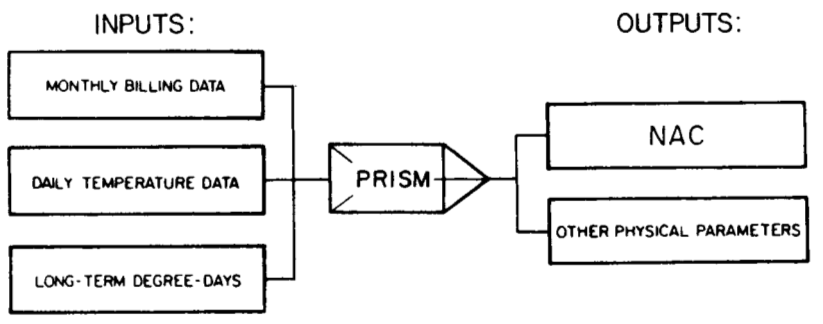
\includegraphics[width=0.5\textwidth]{images/prism.png}
  \caption{Prism flow diagram}
  \label{fig:prism}
\end{figure}
\FloatBarrier

The model have three physically meaningful output: base-load reflects
the consumption of appliances, reference temperature reflects the
setpoint temperature, slope reflects the ``lossiness'' of the house
(heat-loss rate in the heating model). The reference temperature is
affected by the indoor temperature setpoint.
% \begin{figure}[h!]
%   \centering
%   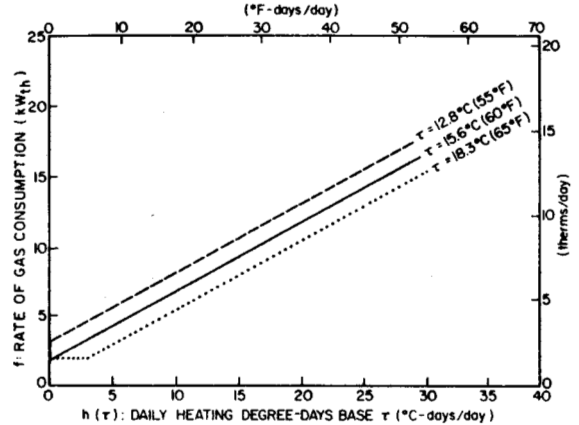
\includegraphics[width=0.5\textwidth]{images/prismDDchange.png}
%   \caption{Degree base change influences energy consumption for a idealized house}
% \end{figure}
% \FloatBarrier

The model assumes a proportional increase in heating energy
consumption when the temperature is below some threshold.  The
reference temperature is chosen so that the energy-degree day plot is
closest to a straight line, with the highest $R^2$ or the least mean
squared error.
\subsection{Baselining methodology for facility-level monthly energy
  use-part 1: Theoretical aspects~\cite{reddy1997baselining}}
The paper proposed a baseline methodology for ECM saving calculation
and ``determine progress toward any preset energy-efficiency goals''
calculation at the facility level. The paper compared the performance
of two software packages: PRISM by Fels et al.\ (using VBDD), and
EModel by Kissock et al.\ (using simple regression with Monthly Mean
Temperature);discussed the baseline year selection rule; and proposed
statistical methods for evaluating uncertainties.

The paper listed a few building energy conservation programs supported
by Executive Order 12902 (reducing 30\% energy per gross square foot
from 1985 to 2005): Federal Energy Management Program (FEMP), Rebuild
America, and Energy Star. The paper is part of the the Model Energy
Installation Program (MEIP).

The author summarized potential influential variables of building
energy consumption: 1) climate, 2) conditioned area, 3) occupancy, 4)
non-ECM related load, 5) ECM related load. The paper only normalizes
for 1) and 2) and uses baseline selection rule to isolate the effect
of 5).

The input variables are outdoor dry-bulb temperature (claimed to be
the most influential independent variable), and monthly utility
bills. The method provides the error band for both the monthly and the
annual level, and a solution for un-known utility reading dates. One
reason for not including occupancy in the model is that it is usually
not measured well.

The model evaluation / selection measure (goodness of fit) used are
$R^2$ and CV-RMSE. $R^2$ describes the variation in the dependent
explained by the model. It indicates ``how well the model fits the
data''. CV-RMSE (in \%) is a form of normalized $RMSE$. It is suitable
if the aim is to calculate the energy saving. The formula of CV-RMSE
here and in the ASHRAE standard has $n - p$ ($n$: sample size, $p$:
number of parameters) in the denominator, but I'm not sure if this is
appropriate, same with standard deviation. The author argues that the
criteria of $R^2 >0.1$ and CV-RMSE $< 7\%$ be deemed ``good'' models
proposed by Fels et al.\ is arbitrary. There should not be a strict
cutoff. The criteria used in this paper is also arbitrary: CV-RMSE
less than 5\%, 10\%, 20\% are considered excellent, good, and mediocre,
CV-RMSE $> 20\%$ is considered poor. Standard error (SE) measures
``how accurately the regression model is able to identify the
individual model coefficients''.

For the VBDD method, it is most suitable for single-zone buildings
(residential, or small commercial). The inputs of the associated
package are monthly utility bill, and daily average outdoor
temperature and outputs normalized annual consumption (NAC), the
energy consumption under average weather conditions, and $R^2$. The
saving is calculated by $NAC_{pre} - NAC_{post}$, the model is in the
form of \eref{eq:vbdd-1}($DD(\tau)$ is either heating or cooling
degree day), and \eref{eq:vbdd-2} ($_h$ for heating, $_c$ for
cooling). The $Y$ are monthly mean daily energy, not monthly total
energy.
\begin{equation}
  \label{eq:vbdd-1}
    Y = \alpha + \beta \cdot DD(\tau)
\end{equation}
\begin{equation}
  \label{eq:vbdd-2}
    Y = \alpha + \beta_h \cdot DD(\tau_h) + \beta_c \cdot DD(\tau_h)
\end{equation}

For the Simple Regression Models Using Monthly Mean Temperature (MMT),
the author emphasized that the temperature should be during the same
period as the billing period, not the calendar month. The 1 to 5
parameter models are:
\begin{equation}
  \label{eq:p1}
    Y = \bar{T}
\end{equation}
\begin{equation}
  \label{eq:p2}
    Y = \alpha + \beta \cdot T
\end{equation}
\begin{equation}
  \label{eq:p3a}
    Y = Y_{cp} + RS \cdot (T - X_{CP})^+
\end{equation}
\begin{equation}
  \label{eq:p3b}
    Y = Y_{cp} + LS \cdot (T - X_{CP})^-
\end{equation}
\begin{equation}
  \label{eq:p4}
    Y = Y_{cp} + RS \cdot (T - X_{CP})^+ + LS \cdot (T - X_{CP})^-
\end{equation}
\begin{equation}
  \label{eq:p5}
    Y = Y_{cp} + RS \cdot (T - X_{CP, h})^+ + LS \cdot (T - X_{CP, c})^-
\end{equation}
The form of the 3 to 5 parameter enforces the different pieces to be
continuous. The package by Kissock et al.\ implemented these models
better suitable for hourly or daily data for commercial buildings, but
could be used on monthly data (suitable for hourly is
doubtful). \cite{haberl1994bin} is to be further read to checked for
the implementation details of the package. The inputs to the package
are: monthly mean daily temperature, and the monthly utility bill.

The author discussed the uncertainty of the MMT models. The standard
approaches for computing the 90\% confidence band for the
(non-segmented) linear regression does not apply to 3 to 5 parameter
change point models, because they are not linear. The authors also
found that the residuals for a 3P MMT model have different variance on
different sides of the change point. The authors claimed the standard
testing method for the MMT models are too complicated to be feasible,
but this needs to be further checked. They propose to compute a
separate 90\% confidence band for different segments in the piecewise
regression regression. Although the description of $X_0$ is
confusing. The annual confidence interval equals the average of the
monthly ones.

The author pointed out the uncertainty of bill reading date could
result in some inaccuracy in the saving estimate, and proposed a
method to estimate the approximate reading date: computing a model for
each potential utility bill reading time and choose the best model
with low CV-RMSE. Although since the reading dates of one month
influence the calculation of adjacent months, one would probably want
to optimize for the aggregated CV-RMSE for all months, instead of just
one month.

\subsection{Comparisons of inverse modeling approaches for predicting
  building energy performance~\cite{Zhang2015177}}
The paper reviewed four major data-driven energy baseline models for
building energy prediction, in the context of ECM saving calculation.
The application of such models include ``determining retrofit savings,
energy system fault diagnostics, and acquiring physical insight into
the operating patterns''~\cite{Zhang2015177}, ``control strategy
development, and on-line control applications''~\cite{Zhang2015177}.

The author briefly listed some existing data-driven baseline methods
including: constant base degree day method, variable-base degree day
method, degree-hour method for heating and cooling energy demand
prediction, the bin model (compares pre and post retrofit average
hourly energy consumption for the 24 hour of the day), ANN models,
generalized fourier series model, support vector machine regression
model Pulse Adaptive Model, change-point model, LBNL model,
mean-week-model, day-time-temperature-model, decision tree method.

Gaussian Process Regression method, Gaussian Mixture Regression Model,
are proposed and are compared with change-point regression model and
an ANN based model.

The four methods are tested on an office building data to predict the
hot water energy consumption with $R^2$, RMSE, CV-RMSE. For the hourly
prediction, the data from 2012-1-1 to 2012-2-24 is selected as the
training set, and the data from 2011-12-8 to 2011-12-31 is used as the
test set. For the daily prediction, 2012-1-1 to 2012-12-5 is selected
as the training set, and the 2011-8-11 to 2011-12-31 is the test
set. The rational for the selection of the size of training set is not
mentioned.

The input is the dry-bulb temperature. The author also have tested
adding HVAC hour of operation, and horizontal heat flux are also tried
out, but claimed that these two additional variables did not have much
impact and were thus dropped from the model. (It is not clear how this
step is conducted, seems to lack a solid procedure, the author should
leave those variables in the regression and use regularization terms
to automatically set their weights to be very small or to be zero. Or
maybe using PCA to pre-processing the data)

A three parameter change-point model was learned for both the daily
and hourly model. However, the equation (10) and the plot (figure 7)
does not match, as the intercept in the plot does not match that of
the equation: the function in equation (10) is not continuous, while
the plot is. unless the unit for power demand is also a different from
the equation (the equation seems to have used degree F and plot used
degree C, which is confusing). This implicit assumption will needs
further researching on.

For the change-point model, the author explained the algorithm for
finding the change point, and commented that the method is ``good for
its simplicity, robustness and accuracy''. However, this claim does
not have any evidence presented here, especially robustness and
accuracy.

The author discovered that for the change point model, the hourly
model have more ``error'' and provided the following explanation:
``hourly building behavior usually has instant large energy flow
demands, which cannot be respond immediately by the HVAC system due to
relatively high system inertia''... ``This system inertia could
contribute to the error in the training data set''.

The description of the Gaussian process and Gaussian mixture process
models are very confusing, I need further readings other than this
paper in order to understand this part more.

In the conclusion section, the author claims that ANN model is the
worst because ``ANN model needs sufficient training data in order to
accurately capture the relationship''. However, they haven't provided
justification of this, one could have tested the influence of the size
of training data on the performance on the test data. Also, since
there are so many different implementations of ANN, it could be the
case that the authors just implemented a bad one. Also not sure why
the author thinks GMM is the best: GMM is the best in hourly models,
but GPM is actually the best in daily models.

Also in the conclusion, the author wrote, ``all models except the ANN
model (CV-RMSE of 32.35\%)'' meets the ASHRAE standard. It is wrong,
because we want ``CV-RMSE'' to be small, not large, it should be ANN
does NOT meet the standard and other models do.

Some terms are used in-correctly: ``non-negative definite'' should be
``positive semidefinite'', ``priori'' should be ``prior'', in table 6,
the model abbreviations are different from those that are used in the
text (``GMM'' changed to ``GMR'', ``GPM'' changed to ``GPR'')

The author cited that the requirement in ASHRAE guideline are as
\tref{tab:modelerr} follows, but I searched, the 22\%, 5\%, 7\% are
not there.  the places with 10\%:
\begin{itemize}
\item ``The computer model shall have an NMBE of 5\% and a CV(RMSE) of
  15\% relative to monthly calibration data. If hourly calibration
  data are used, these requirements shall be 10\% and 30\%,
  respectively.'' (but this is under the ``Whole-Building Calibrated
  Simulation Performance Path'' though, which is not relevant here)
\item ``baseline model shall have a maximum CV(RMSE) of 20\% for
  energy use and 30\% for demand quantities when less than 12 months’
  worth of postretrofit data are avail- able for computing
  savings. These requirements are 25\% and 35\%, respectively, when 12
  to 60 months of data will be used in computing savings. When more
  than 60 months of data will be available, these requirements are
  30\% and 40\%, respectively'' (this is the relevant one)
\end{itemize}
\begin{table}[h!]
  \centering
  \begin{tabular}{c|c|c|c}
    \hline
    &Monthly &Daily &Hourly\\
    \hline
    \hline
    CV-RMSE&15\%&22\%&30\%\\
    \hline
    NMBE&5\%&7\%&10\%\\
    \hline
  \end{tabular}
  \caption{ASHRAE guideline 14 requirement of model error (wrong)~\cite{Zhang2015177}}
  \label{tab:modelerr}
\end{table}
\subsection{Applying support vector machines to predict building
energy consumption in tropical region~\cite{dong2005applying}}
The paper presented an approach of kernelized SVM regression on
building load forcasting and a general discussion of the feasibility
and parameter estimation approaches of the SVM model. The input
variables include monthly outdoor dry-bulb temperature, relative
humidity, global solar radiation, and monthly utility bill. The
utility bills are collected from survey data, and the weather data are
received from the Singapore National Environment Agency.

The paper defined the landlord energy consumption as the energy used
in central ventilation and air-conditioning system, vertical
transportation, and lighting. The authors argues that the landlord
energy should be used in ECM saving calculation instead of the whole
building. The fact that landlord energy consumption has non-linear
components motivates this study of the non-linear models for energy
consumption estimation.

The primal objective function form of SVM can be expressed as:
\begin{equation}
  \label{eq:svm}
  \frac{1}{2}\left\|w\right\|^2 + C \sum_{i = 1}^nL_{\epsilon}(y_i, \hat{y_i})\\
\end{equation}
\begin{equation}
  L_{\epsilon} = \begin{cases}
    \left|y_i - \hat{y_i}\right| - \epsilon &\text{if $\left|y_i - \hat{y_i}\right| > 0$}\\
    0 &\text{otherwise}
    \end{cases}
\end{equation}
The $L(y_i, \hat{y_i})$ is the the $\epsilon$ insensitive loss
function. The Lagrangian dual of the SVM regression is kernelizable,
and could be more probable to achieve large margin in the higher
dimensional $\phi$ space, thus prevents over-fitting. It also models
the non-linear component in the regression model. The loss function is
measuring the structural risk, which corresponds to ``an upper bound
of the generalization error''. The author pointed out that input
should be scaled to $[-1, 1]$ or $[0, 1]$ before applying SVM or ANN.
This could reduce numerical error, and balance the influence of
different variables.

The parameters $C$ and $\epsilon$ in the objective function are
selected with 3-fold cross validation (selecting $\gamma$, a one-time
search method~\cite{cao2003support} (searching for $C$, and
$\epsilon$), and stepwise search (a more efficient variation of the
grid search for $C$ and $\epsilon$). In the classification setting,
$C$ represent the trade-off between allowing large margin, and the
amount of mis-classification. Larger $C$ will more strictly penalize
mis-classification, and small $C$ will favors large margin. In the
regression setting, $C$ controls the tradeoff between model complexity
and ``model complexity and the degree to which deviations larger than
$\epsilon$ are tolerated''. Larger $\epsilon$ corresponds to sparser
solution but could also harm the accuracy. Each building has its own
set of parameter values. Brown et al.\ commented that ``their technique lacks a
continuous optimization framework for kernel bandwidths
and cannot generalize to large training sets''~\cite{brown2012kernel}.

The method is tested on 4 randomly selected commercial office
buildings from the central area of Singapore in CV-RMSE, and error\%
($\frac{\hat{Y} - Y}{Y}$). In the testing, the $MSE$ ranges between
0.14 to 0.73, but the CV-RMSEs are all less than 5\%. However, the
author compared the proposed method with other methods without stating
the difference in the number of input variables, and the difference
in time resolution. The mere comparison of CV-RMSE thus renders
meaningless. Also using $CV$ to indicate CV-RMSE is not good, because
it is usually reserved for cross-validataion. The author further
brought about the issue of residual does not follow normal
distribution, but claimed that it is at least consistent (the errors
seems to be independent).

The author summarized the advantage of SVM: 1) It
minimizes the upper bound of the generalization error, instead of just
training error. This ensures a better generalization guarantee in the
unseen data. 2) the objective function is convex, so the local optimal
is the global optimal. 3) It could provide a sparse solution, where
the learned model can be represented by only a small subset of the
input data. The authors selected the RBF kernel in the model as it can
model non-linear relation, and is simpler with fewer hyper
parameters. 4) It performs well even when the number of training data
is small (4 year utility bill).

\subsection{Kernel regression for real-time building energy
  analysis~\cite{brown2012kernel}}
The authors proposed kernel regression method hourly building energy
signature modeling. In terms of predictive power, it outperforms
conventional neuron network models, especially for cases where the
size of training data is small, and in terms of interpretability, the
model coefficients (bandwidths) encodes the importance of the
corresponding parameter, which could in turn give insights about the
physical condition of target building: the most relevant time scale
for temperature reflects the thermal inertia (insulation and thermal
mass); the importance of the wind factor corresponds to the height of
the building with respect to surrounding buildings. On the other hand,
the weights in neuron network models are generally meaningless. Also
since the number of parameters are smaller than neuron network, kernel
regression is less prone to overfitting (\fref{fig:overfitKernel}). It
could also prevent outputing infeasible solutions such as predicting
negative energy consumption. It performs especially well in buildings
with complex non-linear behaviour.
\begin{figure}[h!]
  \centering
  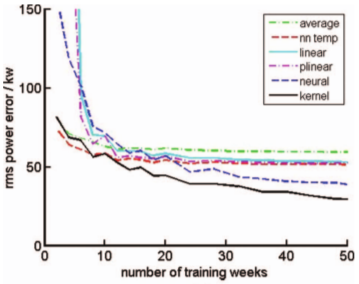
\includegraphics[width=0.5\textwidth]{images/overfitKernel.png}
  \caption{Comparing rms of test set by number of train data}
  \label{fig:overfitKernel}
\end{figure}

In order to be applied to a large building portfolio, the authors
pointed out that a good model should be more scalable and
deployable. Acquiring the physical details and tuning the parameters
in the calibrated simulation approach could be difficult for large
building portfolio, and simpler models with looser physical basis
becomes increasingly popular. In general, these energy models could be
useful in building energy system diagnostics, fault or event
detection, smart building control, and building energy retrofit saving
calculation. The model presented in this study aims to tackle energy
prediction and peak power event detection.

The author summarized a list of models developed since last 90s. For
the black box models with no physical basis, a lot of neuron network
based algorithms were developed, ranking top during both phases of the
ASHRAE `Great Energy Predictor Shootout' competition. The winner
methods are: Mackay's baysian modeling with neuron
network~\cite{mackay1996bayesian} in phase I, and the method of Dodier
and Henze~\cite{dodier2004statistical} in phase II. To determine which
input variables are more relevant, the former used a Automatic
Relevance Determination (ARD) prior, and the latter used the Wald's
test~\cite{dodier2004statistical}. After the competition, work have
been done in frequency domain modeling, online neuron networks, SVM
regression, etc.. For the grey-box models with simplified building
physical specification, parameters are estimated from the data by
maximizing likelihood or minimizing loss. Two example are presented:
\cite{andersen2000modelling}, and \cite{lee2004development}.

For the proposed method, there are 4 input variables to the model:
time, temperature, humidity, and wind velocity. The input variables
are transformed to 14 features before fed to the model. The time input
is transformed to 8 parameters of four scales with
\eref{eq:timeCircle}
% fixme
\begin{equation}
  \label{eq:timeCircle}
  [\cos (\frac{2\pi t}{T}), \sin (\frac{2\pi t}{T})]
\end{equation}
The temperature, humidity, and wind hourly inputs are transformed with
exponential weighting functions. Before the transformation, the inputs
are normalized with mean and standard deviation. Separate models of
weekday, weekend, and holidays are trained.

Kernel regression or kernel smoothing method makes prediction with a
``weighted average of nearby data items, with the weights being
controlled by a kernel function''~\cite{brown2012kernel} (Gaussian
kernel with diagonal covariance in this study \eref{eq:gaussianKernel}).
\begin{equation}
  \label{eq:gaussianKernel}
  k(\mathbf{x}, \mathbf{x_i}) = \mathcal{N}(\mathbf{x} - \mathbf{x_i}; 0, diag(\mathbf{\sigma}^2))
\end{equation}
% fixme what is the covariance matrix
(it might mean this form
$k(x, x_i) = \exp(-\frac{\left\|\mathbf{x} - \mathbf{x_i} -
    0\right\|^2}{2\sigma^T\sigma}))$)

In the training stage, the objective or the L2 loss function (mean
squared error) is minimized with respect to $\mathbf{\sigma}$ (the
vector of bandwidths) using cross-validation. An approximation
approach is adopted to increase the computation efficiency by keeping
only the nearest k data points in the summation). 
\begin{equation}
  \label{eq:l2}
  loss = \frac{1}{\left|S\right|}\sum_{i = 1}^{\left|S\right|}(y_i - \hat{y_i})^2
\end{equation}

The method is tested with two data sets: the ASHRAE Predictor Shootout
dataset, and another data set of 4 buildings with 1.5 year of hourly
electricity and environment inputs. It is compared with a few other
baseline models: Temporal average, Temperature neighbours,
Multivariate linear, Piecewise linear, and Neural network. For
multivariate linear and piecewise linear models, a separate model is
learned for each hour of the day, and for weekdays, and weekends. 

With the 1.5 year data set, every 1st and 2nd week of the 1.5 year
data (52 weeks total) is selected as the training set, and every 3rd
week of the 1.5 year data (26 weeks total) is held out as the test
data set. The performance of different methods are evaluated with
CV(RMSE).
training data.
\begin{figure}[h!]
  \centering
  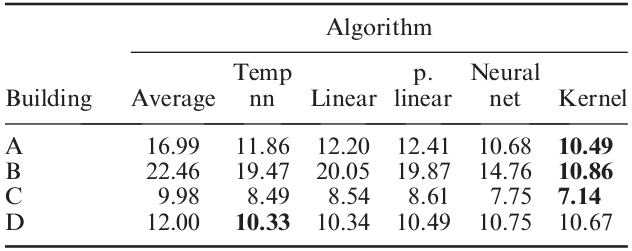
\includegraphics[width=0.5\textwidth]{images/kernelResultCmp.png}
  \caption{Test result}
  \label{fig:ker}
\end{figure}

With the ASHRAE data set, the method is compared with other top
ranking methods in the competition. It is comparable to other neuron
network approaches, but is worse than the top method. The authors
propose future works could include 1) using L1 loss function to
enforce a sparse solution, 2) include automatic parameter selection
(PCA maybe?), and 3) testing on larger building portfolio.

This paper provides a clear guidance of the model design and testing
procedure. It also contains useful information about implementation
tricks, which could help in further model implementation design.

\subsection{Contextually Supervised Source Separation with Application
  to Energy Disaggregation~\cite{wytock2013contextually}}
The paper presented a solution to single-channel source separation
problem (decompose an observed signal to several un-observed component
signals) under the motivation of ``energy disaggregation of hourly
smart meter data''. The method is tested on a large scale: thousands
of homes. The data for supervised setting is difficult to get, and the
un-supervised setting is ill-defined and has arbitrarily many
solutions. Thus the authors proposed a hybrid approach of contextual
supervised setting. The ``contextual features'' are features that
influences the un-observed signals, environment variables in the
application of building energy disaggregation. They proved that under
the condition that the contextual features for different hidden signal
components are roughly linearly independent, then the method achieves
high accuracy with high probability.

The input to the method include: 15-min or hourly power meter data,
collected from PG\&E by the utility from Northern California
homes. The context feature is temperature, retrieved from Weather
Underground with census block level addresses. Radial-bases functions
(RBFs) are used on the non-linear relationship between temperature and
energy. The energy are disaggregated into four categories: base
(time-of-day dependent), cooling, heating, and other
(featureless). $l_1$ loss function is used for all components, but for
heating and cooling energy, a smoothing matrix ($S_n$) is used to
model the ``lag effect''.

The problem is formalized as an optimization:
$$
\begin{aligned}
  \label{eq:opt}
  &\underset{Y, \theta}{\text{minimize}} &&\sum_{i = 1}^k {l_i (y_i , X_i \theta_i) + g_i(y_i) + h_i(\theta_i)}\\
  &\text{subject to} &&\sum_{i = 1}^k y_i = \bar{y}\\
\end{aligned}
$$
$X_i$ is the bases specific to each hidden signal component. $Y$ is
the matrix whose columns are the decomposed signals
$Y = [y_1, \dots, y_k]$, $l_(\cdot, \cdot)$ is the loss function
measures the difference between the predicted value and the true
signal. $g_i$ is a regularization term for $y_i$, and $h_i$ is a
regularization term for $\theta_i$. In energy disaggregation
application, the $h_i$ could be dropped since $T \gg n_i$. If all
three terms in the objective function are convex, then the problem
became a convex optimization. In the setting of energy disaggregation,
$l_i$ is in the form of to account for the ``lag'' effect of
temperature on heating / cooling energy consumption ($T$ is the width
of the sliding window). ``air conditioning is correlated with high
temperature but does not respond to outside temperature changes
instantaneously; thermal mass and the varying occupancy in buildings
often results in air conditioning usage that correlates with high
temperature over some window''
\begin{equation}
  \label{eq:loss}
  l_i(y_i, X_i\theta_i) = \left\|(y_i - X_i\theta_i)(I \otimes 1^T)\right\|
\end{equation}
\begin{figure}[h!]
\centering
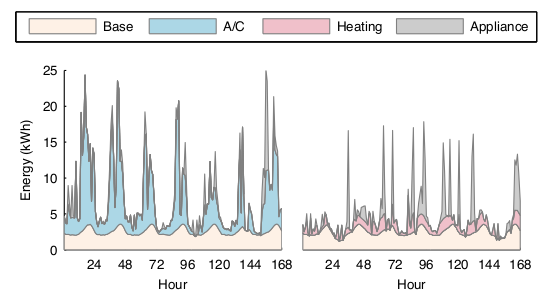
\includegraphics[width=0.7\textwidth]{images/disagg.png}
\caption{Disaggregation of energy use for a home in CA}
\label{fig:dis}
\end{figure}

\begin{table}[h!]
  \centering
  \begin{tabular}{c|c|c|c}
    \hline
    Category&Features&$l_i$&$g_i$\\
    \hline
    Cooling&Hour of day&$\left\|y_1 - X_i\theta_1\right\|_1$&$\left\|Dy_i\right\|_2^2$\\
    Cooling&RBFs over temperature $> 70^oF$&$S_2\left\|S_2(y_2 - X_2\theta_2\right\|_1$&$0.1 \times \left\|Dy_2\right\|_1$\\
    Heating&RBFs over temperature $< 50^oF$&$S_2\left\|S_2(y_3 - X_3\theta_3\right\|_1$&$0.1 \times \left\|Dy_3\right\|_1$\\
    Other&None&$\left\|y_4\right\|_1$&$0.5 \times \left\|Dy_3\right\|_1$\\
    \hline
  \end{tabular}
  \caption{model specification for the test data}
  \label{tab:dis}
\end{table}
The $RBF$ is an approximation of the function approximation of the
temperature~\cite{elair}.

The method is validated on a data set of 84 homes with at least 1 year
hourly (rolled up from one-minute interval raw data) electric usage in
Texas. The proposed method has outperformed the mean prediction
heuristic (Mean) and a state-of-the art unsupervised method, sparse coding (NNSC),
in this test set.

\begin{table}[h!]
  \centering
  \begin{tabular}{c|c|c|c}
    \hline
    Category&Mean&NNSC&Contextual (proposed method)\\
    \hline
    Base&0.2534&0.2793&0.1849\\
    A/C&0.2849&0.2894&0.1919\\
    Appliances&0.2262&0.2701&0.1900\\
    Average&0.2584&0.2701&0.1889\\
    \hline
  \end{tabular}
  \caption{Comparison of performance on Pecan Street
dataset, measured in mean absolute error (MAE)}
\label{tab:maeContext}
\end{table}
The method is then applied on a large-scale 4000+ home setting and
estimated 15.6\% of energy consumption is used in air conditioning and
7.7\% to heating in the disaggregation result. It is reasonably close
to survey result from EIA 2009 (10.4\% for air conditioning and 5.4\%
for space heating)

The biggest difference of this method 1) it has performance guarantee
through proof 2) it is tested against a large data set and benchmarked
with other methods.
\subsection{Deep learning for estimating building energy
  consumption~\cite{mocanu2016deep}}
% note: good point: tested on various time ranges
The authors proposed two deep-learning based energy models:
Conditional Restricted Boltzmann Machine (CRBM) and Factored
Conditional Restricted Boltzmann Machine (FCRBM). The authors provided
briefly mentioned the some existing approaches of hybrid (grey-box)
energy models: semi-parametric regression models, exponential
smoothing, seasonal time series models.

The proposed CRBM model and FCRBM model are explained in three aspects:
the energy function, probablistic inference, and the updating
rule. The input to the models are the energy time-series. Environment
factors are not included.

The models are tested against ANN, SVM, and Recurrent Networks on the
``Individual household electric power consumption'' data set with 4
years of one-minute electric data (including about 1\% missing data)
with three sub-meters and one whole house meter. The first three years
is selected as the training set, and the last year's data is the test
set.

The models are evaluated with root mean squared error (RMSE),
correlation coefficient ($R$), and p value of the hypothesis test
against ``predicted and real data are unrelated''.

Some pre-processing are conducted before the training and testing: the
missing data is filled with the average of data at the same date-time
of the other years.

As the deep learning is one of the current hot and state-of-the art
technique, and it made to the front page of New York
Time~\cite{mgormley2016}, it is worth reviewing its application in the
field of building energy. Although the work in this paper is in the
context of smart-grid and demand side control, the predictive model
will still be helpful in the identification of the energy retrofit
opportunities, and saving calculation. The deep neuron nets needs to
be further digested if it was to be implemented, as the model seems to
be a bit complicated. There are some limitations to the study: the
model is evaluated on one building.
\subsection{A decision tree method for building energy demand
  modeling~\cite{Yu20101637}}
The authors developed a decision tree based method to predict energy
consumption (??). The advantage of the method is its result is more
interpretable with a tree structure. It is demonstrated by estimating
the ``energy performance index'' (or EUI?) of 67 residential buildings
in 6 districts of Japan. The accuracy is 93\% for the training data,
and 92\% for the test data. It could also rank the EUI influential
factors automatically.  The authors mentioned methods of building
energy demand modeling: traditional regression, ANN, simulation, and
pointed out the drawback of regression method and ANN are they are not
easily interpretable. Also they are only applicable to existing
buildings. Simulation methods have less predictive power for occupied
buildings and also too complicated~\cite{Yu20101637}.

The author briefly described the structure of decision tree (what do
the nodes and edges represent), and the procedure for learning a
decision tree. A more thorough description could be found in Tom
Mitchell's book.

The author also mentioned some commonly methods for learning a
decision tree: ID3, CART, and C4.5 (used in this study). The tool WEKA
is used in the implementation.

In the demonstration example, the target to be predicted is
categorical: High EUI, or Low EUI. The cutoff is the average of the
max and min EUI of the data set. The input data include energy
consumption of electricity, natural gas, and kerosene (5 min
interval), 15min indoor environment, building characteristics, and the
number of occupant. The numerical temperature is converted to
categorical with low temperature being 8.8C to 13.1 C, and high
temperature being 14.3C to 17.4C. The building characteristics include
house type (detached or apartment), construction (wooden vs
non-wooden), floor are, heat loss coefficient, and equivalent leakage
area.

The learned model is shown in the following.
\begin{figure}[h!]
  \centering
  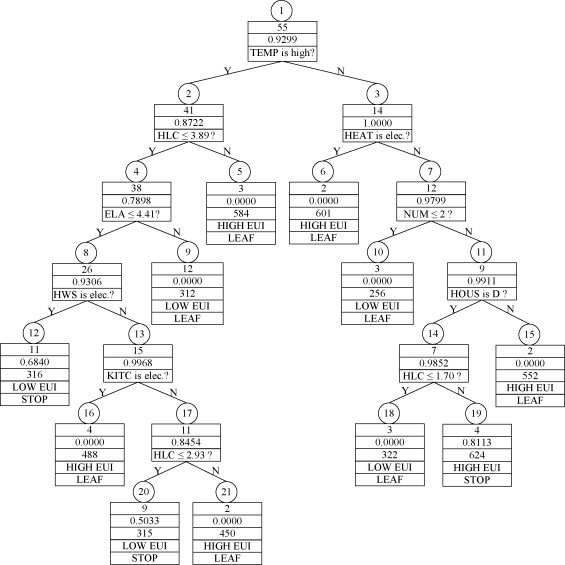
\includegraphics[width=0.5\textwidth]{images/decisionTreeLeared.jpg}
  \caption{The learned decision tree model~\cite{Yu20101637}}
  \label{fig:decisionTreeLeared}
\end{figure}
\FloatBarrier 

Two points are not clear:
\begin{itemize}
\item What is the reference EUI: the model is a classifier, how could it
output a numeric value, if it can, why predicting a category instead
of the actual consumption?
\item How is the confidence level computed?
\end{itemize}

The author claimed that a rank of importance of the influential
factors can be extracted from the model: the root node is the most
important factor, the closer a node is to the root, the more important
the factor is. However, I have doubts about this, the selection of the
spliting factor at each level, as the author mentioned, is based on
the ``information gain''. If the ``information gain'' indicates the
rank of importance needs further research. Nevertheless, the authors
reached some interesting interpretations of the learned decision tree
model: temperature (indoor) is the most important factor; the tree is
not symetric, meaning different factors are found important in the
high and low temperature group; in the high-temperature (indoor)
group, high heat loss coefficient and equivalent leakage are
corresponds to high EUI, etc.
\begin{table}[h!]
\centering
\caption{Rank of factors}
\label{tab:rank}
\begin{tabular}{l|p{3cm}|l|p{3cm}|l}
  \hline
Potential factors       & High temperature districts &                           & Low temperature districts& \\
                        & Significant factors        & Rank                      & Significant factors & Rank \\
  \hline
  \hline
House type              &                            &                           & \cmark              & 3    \\
  \hline
Number of occupants     &                            &                           & \cmark              & 2    \\
  \hline
Floor area              &                            &                           &                     &      \\
  \hline
Heat loss coefficient   & \cmark                     & 1                         & \cmark              & 4    \\
  \hline
Equivalent leakage area & \cmark                     & 2                         &                     &      \\
  \hline
Construction type       &                            &                           &                     &      \\
  \hline
Space heating mode      &                            &                           & \cmark              & 1    \\
  \hline
Hot water supply mode   & \cmark                     & 3                         &                     &      \\
  \hline
Kitchen energy mode     & \cmark                     & 4                         &                     &      \\
  \hline
\end{tabular}
\end{table}

There's a comparison between the influence of water heater fuel type
on EUI with HLC and ELA controled \fref{fig:cmpHWS}. The author argued
that generally, the red points are higher than the blue
points. However there's a bit confusion here, as what do the line
segments represents. 
\begin{figure}[h!]
  \centering
  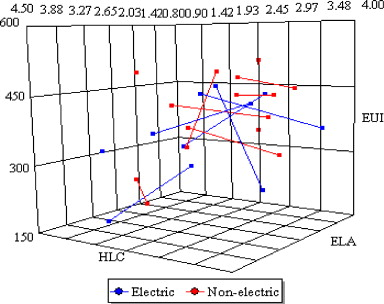
\includegraphics[width=0.4\textwidth]{images/cmpHWS.jpg}
  \caption{The comparison between electric and non-electric water heater on EUI~\cite{Yu20101637}}
  \label{fig:cmpHWS}
\end{figure}
\FloatBarrier Another comparison of the fuel type of space heating
also showed high EUI tends to associate with electric heating.
\begin{figure}[h!]
  \centering
  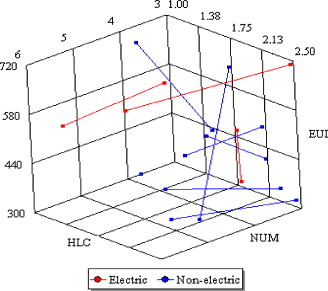
\includegraphics[width=0.4\textwidth]{images/cmpSpace.jpg}
  \caption{The comparison between electric and non-electric space heating (HEAT) on EUI~\cite{Yu20101637}}
  \label{fig:cmpSpace}
\end{figure}
\FloatBarrier 

\subsection{Evaluation of the Predictive Accuracy of Five Whole
  Building Baseline Models~\cite{granderson2014evaluation}}
This paper compared the predictive performance of five whole building
energy baseline methods: Pulse Adaptive Model (PAM), multi-parameter
change-point, mean-week, day-time-temperature, and LBNL models, and
showed that the PAM, day-time-temperature, and the LBNL perform better
then the other two models. The evaluation metrics include: median
absolute percent error, correlation (??), root mean squared error, and
relative bias.

\subsection{Something about RNN}
\subsection{Machine Learning~\cite{mitchell1997machine}}
\subsubsection{Neuron network}
\subsubsection{Decision tree}
\subsection{Bishop book}
\subsubsection{Regression}
\subsubsection{SVM}
\subsection{Boosting}
The paper explains boosting with an example of distinguishing spam
from non-spam emails. The method rises from the observation that it is
easier to create a ``weak learner'' (base learning algorithm) that
finds some rough rules then to find a single accurate procedure. By
repeatedly calling the ``weak learners'' on subsets of data, a lot of
rough rules are generated. After T iterations, the boosting combines
the weak rules with a weighted majority vote. The subsets are chosen
so that the weak learner focuses on ``hard'' examples.
\subsection{Saving Electrical Energy in Commercial Buildings
  ~\cite{case2012saving}}
The thesis develops a method to predict operating parameters with
hourly electric meter data. The operating parameters are a set of
operating modes, each containing a peak and a base with average start
and end times, and a regression model~\cite{case2012saving}. These
operating parameters can be used for energy consumption prediction,
saving calculation, portfolio benchmarking, etc. The method is tested
on 10 buildings with 21 years of energy data, against the method ??.
\subsection{Forecasting Energy Demand in Large Commercial Buildings
    Using Support Vector Machine Regression}
% \section{Methodology}
% \section{Conclusion}
% \begin{itemize}
% \item Suggestions in model evaluation metric
% \item Which method (in history, or the one proposed in the study) works better
% \end{itemize}
\begin{comment}
\section{List of articles}
a list to look at (cited the paper ``Baselining Methodology forFacility-Level Monthly EnergyUse—Part 1: Theoretical Aspects''):
\url{https://scholar.google.com/scholar?client=ubuntu&channel=fs&oe=utf-8&um=1&ie=UTF-8&lr&cites=12191769260004236330}
\begin{itemize}
\item
  \href{http://www.sciencedirect.com/science/article/pii/036013239090020R}{Assessment
    of the energy savings due to the building retrofit} Normalized
  energy consumption is calculated using the ``energy signature''
  (developed from predictions of the daily energy use along with the
  daily average outdoor temperature) and the number of hours of
  occurrence of different outdoor temperature bins for the same
  reference year. Savings due to the building retrofit are obtained as
  the difference between the normalized energy consumptions before and
  after retrofit. The method is compared with DOE-2 model
\item \href{http://eetd.lbl.gov/sites/all/files/lbnl-23674_0.pdf}{A
    Comparison of Weather Normalization Techniques for Commercial
    Building Energy Use}
\item \href{http://ieeexplore.ieee.org/document/43201/}{Modeling and
    weather-normalization of whole-house metered data for residential
    end-use load shape estimation}weather-dependent component is
  modeled as a nonlinear dynamic system based on thermodynamic
  principles
\item
  \href{http://www.sciencedirect.com/science/article/pii/S0140988316000062}{Climate
    normals and weather normalization for utility regulation} Discuss
  the use of different types of climate normals
\item ASHRAE Standard and related documents
\end{itemize}
\end{comment}

\newpage
\bibliographystyle{plain}
\bibliography{myCitation}
\end{document}